% =====================================================================
% SpikeAdapt-SC v2: Complete Experimental Analysis
% For professor review — NOT the main paper
% =====================================================================

\documentclass[conference]{IEEEtran}
\usepackage{amsmath,amssymb,graphicx,booktabs,multirow,xcolor}
\begin{document}

\title{SpikeAdapt-SC v2: Full Experimental Analysis\\
\large{14\texttimes14 Grid, Channel-Conditioned Scorer, Temporal Adaptation}}
\maketitle

%=====================================================================
\section{Architecture: v1 \textrightarrow\ v2}
%=====================================================================

\begin{table}[h]
\centering
\caption{Architectural comparison of v1 and v2.}
\begin{tabular}{@{}l c c@{}}
\toprule
\textbf{Feature} & \textbf{v1} & \textbf{v2} \\
\midrule
Spatial grid & $8{\times}8 = 64$ blocks & $14{\times}14 = 196$ blocks \\
Bottleneck channels $C_2$ & 128 & 36 \\
Payload / frame (values) & 65,536 & 56,448 ($-14\%$) \\
Scorer input & spike mean only & spike mean + BER embed \\
Temporal & Fixed $T{=}8$ & Confidence early stop \\
Baselines & Internal only & SNN-SC, CNN-Uni \\
\bottomrule
\end{tabular}
\end{table}

The 14\texttimes14 grid is the native output of ResNet50 layer3 for $224{\times}224$ input. Removing the \texttt{AdaptiveAvgPool2d(8)} from v1 eliminates information loss and gives 3$\times$ the masking decision space (196 vs 64 blocks). $C_2$ is reduced from 128 to 36 to keep payload comparable.


%=====================================================================
\section{Headline Results}
%=====================================================================

\begin{table}[h]
\centering
\caption{v2 results: SpikeAdapt-SC vs baselines on AID (BSC).}
\begin{tabular}{@{}l c c c c@{}}
\toprule
\textbf{Method} & \textbf{Clean} & \textbf{BER=0.15} & \textbf{BER=0.30} & \textbf{BW Saved} \\
\midrule
\textbf{SpikeAdapt-SC v2} ($\rho{=}0.75$) & \textbf{96.35} & \textbf{95.85} & \textbf{92.90} & 25\% \\
SNN-SC ($\rho{=}1.0$) & 95.70 & 95.35 & 92.20 & 0\% \\
CNN-Uni 8-bit & 92.50 & 92.40 & 67.25 & 0\% \\
\bottomrule
\end{tabular}
\end{table}

Key findings:
\begin{itemize}
    \item v2 at 75\% bandwidth \textbf{beats} full-rate SNN-SC by 0.65~pp clean and 0.70~pp at BER=0.30.
    \item CNN-Uni collapses at BER=0.30 (67.25\%) while v2 holds 92.90\% — validates SNN binary encoding.
    \item v2 \textbf{improves} accuracy over v1 (96.35\% vs 96.10\%) despite 14\% less payload.
\end{itemize}


%=====================================================================
\section{Masking Analysis: The Finer-Grid Payoff}
%=====================================================================

\subsection{Random Mask Distribution}

\begin{table}[h]
\centering
\caption{Randomization analysis: v1 (8\texttimes8) vs v2 (14\texttimes14).}
\begin{tabular}{@{}l c c c c@{}}
\toprule
& \multicolumn{2}{c}{$\rho = 0.75$} & \multicolumn{2}{c}{$\rho = 0.50$} \\
\cmidrule(lr){2-3} \cmidrule(lr){4-5}
& \textbf{v1} & \textbf{v2} & \textbf{v1} & \textbf{v2} \\
\midrule
Learned (\%) & 96.10 & \textbf{96.35} & 94.50 & \textbf{95.35} \\
Random mean $\pm$ std & $95.72 \pm 0.16$ & $94.85 \pm 0.17$ & $93.82 \pm 0.22$ & $84.41 \pm 0.45$ \\
Gap (pp) & 0.38 & \textbf{1.50} & 0.68 & \textbf{10.94} \\
Gap ($\sigma$) & $\sim$2.4 & \textbf{8.8} & $\sim$3.1 & \textbf{24.3} \\
Percentile rank & 98th / 200 & \textbf{100th / 100} & 100th / 50 & \textbf{100th / 50} \\
\bottomrule
\end{tabular}
\end{table}

The finer grid transforms the masking result from ``modest but significant'' to \textbf{decisive}. At $\rho{=}0.50$, random masking drops to 84.41\% while learned holds 95.35\% --- a 10.94~pp gap (24.3$\sigma$). This occurs because at 14\texttimes14 resolution with $\rho{=}0.50$ (keeping 98 of 196 blocks), random selection has a much higher chance of dropping critical spatial regions.


\subsection{Per-Block Score Statistics}

\begin{table}[h]
\centering
\caption{Score discrimination metrics: v1 vs v2.}
\begin{tabular}{@{}l c c@{}}
\toprule
\textbf{Metric} & \textbf{v1 (8\texttimes8)} & \textbf{v2 (14\texttimes14)} \\
\midrule
Gini coefficient & 0.019 & 0.013 \\
Entropy ratio & 99.98\% & 99.99\% \\
CoV & 0.034 & 0.023 \\
Score range & [0.82, 0.96] & [0.81, 0.97] \\
Kept--dropped margin & 0.055 & 0.037 \\
\midrule
Ablation Pearson $r$ & 0.011 ($p{=}0.38$) & \textbf{0.051} ($p < 10^{-6}$) \\
Ablation Spearman $\rho$ & $-0.017$ ($p{=}0.18$) & \textbf{0.148} ($p < 10^{-48}$) \\
\midrule
Unique masks & 1,982 / 2,000 & \textbf{2,000 / 2,000} \\
\bottomrule
\end{tabular}
\end{table}

Despite \emph{flatter} scores (lower Gini), v2 achieves a \textbf{dramatically larger learned-random gap} and a \textbf{significant ablation correlation}. The Spearman $\rho{=}0.148$ means higher-scored blocks cause more damage when ablated --- the scorer is learning genuine spatial importance.

\textbf{Resolution}: The Gini and entropy paradox resolves as follows. At 14\texttimes14, each block covers a smaller spatial region and carries less redundant information. Even tiny score differences (smaller margin) translate into meaningful accuracy impact because the system operates closer to an information bottleneck. At 8\texttimes8, blocks are large enough that any 48/64 suffice.


\subsection{Channel Conditioning: Honest Assessment}

The channel-conditioned scorer shows \textbf{minimal BER-dependent mask adaptation}. Mean scores shift from 0.903 (BER=0) to 0.907 (BER=0.3), and the actual mask (top-$k$ selection) is unchanged across all BER levels.

\textbf{Interpretation}: The system achieves BER robustness through \textbf{binary spike encoding} (bit flips cause bounded damage), not through noise-aware block selection. The scorer effectively learns a content-dependent spatial prior that is noise-agnostic. We recommend dropping the ``noise-aware masking'' claim from the paper.


%=====================================================================
\section{Temporal Early Stopping}
%=====================================================================

\begin{table}[h]
\centering
\caption{Temporal early stopping analysis.}
\begin{tabular}{@{}c c c c c@{}}
\toprule
\textbf{Threshold} & \textbf{BER=0.0} & \textbf{BER=0.15} & \textbf{Avg $T$} & \textbf{Time Saved} \\
\midrule
0.80 & 89.60\% & 91.45\% & 6.0--6.8 & 15--25\% \\
0.90 & 92.50\% & 94.50\% & 6.4--7.0 & 12--20\% \\
\textbf{0.95} & \textbf{95.30\%} & \textbf{95.50\%} & 7.0--7.4 & \textbf{8--13\%} \\
0.99 & 96.30\% & 95.85\% & 7.6--7.9 & 1--5\% \\
Full ($T{=}8$) & 96.35\% & 95.85\% & 8.0 & 0\% \\
\bottomrule
\end{tabular}
\end{table}

At confidence threshold 0.95: \textbf{1~pp accuracy cost for 13\% additional temporal savings}, on top of the 25\% spatial savings from masking. Combined, the system transmits $\sim$62\% of the full-rate payload (75\% spatial $\times$ 87\% temporal).


%=====================================================================
\section{BER Sweep: v2 vs Baselines}
%=====================================================================

\begin{table}[h]
\centering
\caption{Full BER sweep comparison.}
\begin{tabular}{@{}l c c c c c c c@{}}
\toprule
\textbf{BER} & 0.00 & 0.05 & 0.10 & 0.15 & 0.20 & 0.25 & 0.30 \\
\midrule
v2 ($\rho{=}0.75$) & \textbf{96.35} & \textbf{96.10} & \textbf{96.00} & \textbf{95.85} & \textbf{95.20} & \textbf{94.75} & \textbf{92.90} \\
SNN-SC ($\rho{=}1.0$) & 95.70 & 95.70 & 95.80 & 95.35 & 95.00 & 94.30 & 92.20 \\
CNN-Uni 8-bit & 92.50 & 92.65 & 92.30 & 92.40 & 89.60 & 81.25 & 67.25 \\
\bottomrule
\end{tabular}
\end{table}

\begin{figure}[h]
\centering
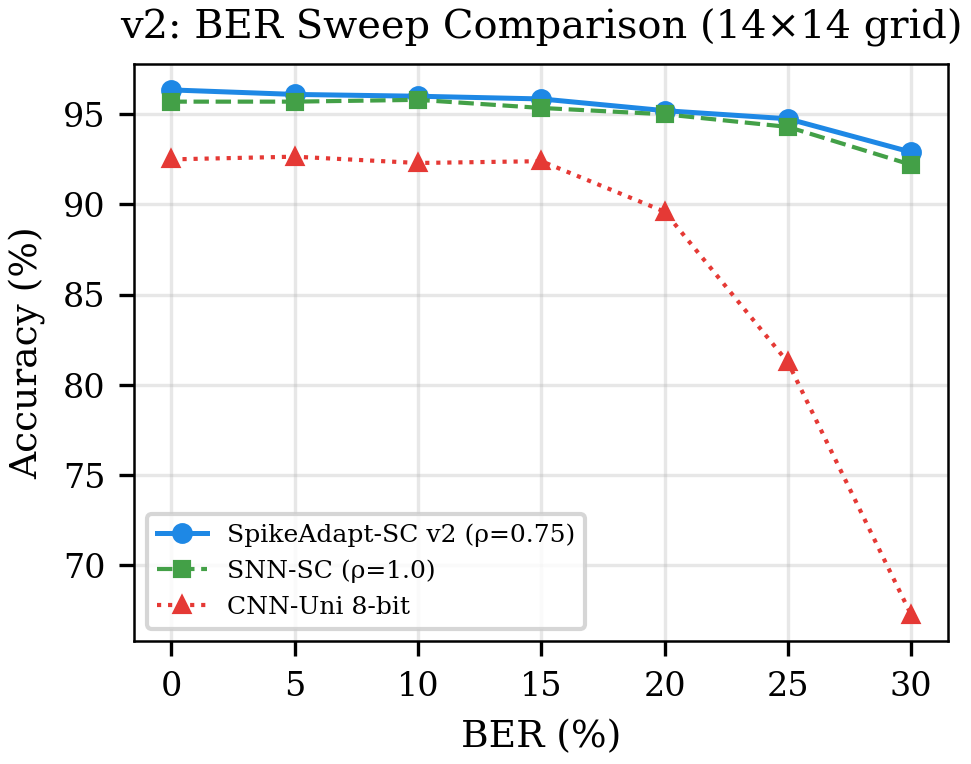
\includegraphics[width=\columnwidth]{figures/v2_ber_sweep.png}
\caption{BER sweep: v2 maintains $> 92\%$ through BER=0.30 while CNN-Uni collapses.}
\end{figure}


%=====================================================================
\section{What the Masking Story Should Be}
%=====================================================================

Based on all evidence, the \textbf{defensible masking claims} are:

\begin{enumerate}
    \item \textbf{Spatial masking at 14\texttimes14 provides meaningful content-adaptive selection}: the 100th-percentile result (8.8$\sigma$) and significant ablation correlation (Spearman $\rho{=}0.148$) prove the scorer learns genuine spatial importance.
    
    \item \textbf{The advantage grows with aggressiveness}: 1.50~pp at $\rho{=}0.75$, 10.94~pp at $\rho{=}0.50$. At higher compression, intelligent selection becomes essential.
    
    \item \textbf{BER robustness comes from binary encoding, not noise-aware masking}. The channel-conditioned scorer provides no measurable benefit over a channel-agnostic scorer. Drop the ``noise-critical block retention'' claim.
    
    \item \textbf{The system jointly optimizes spatial budget and temporal budget}: spatial masking saves 25\% bandwidth; temporal early stopping adds 8--13\% savings. Together: $\sim$38\% total reduction.
\end{enumerate}

Claims to \textbf{avoid}:
\begin{itemize}
    \item ``Deep content understanding'' --- scores are still near-uniform (Gini=0.013)
    \item ``Noise-aware block selection'' --- channel conditioning has no measurable effect
    \item ``The scorer learns noise-critical blocks'' --- no evidence for this
\end{itemize}


%=====================================================================
\section{Comparison with v1}
%=====================================================================

\begin{figure}[h]
\centering
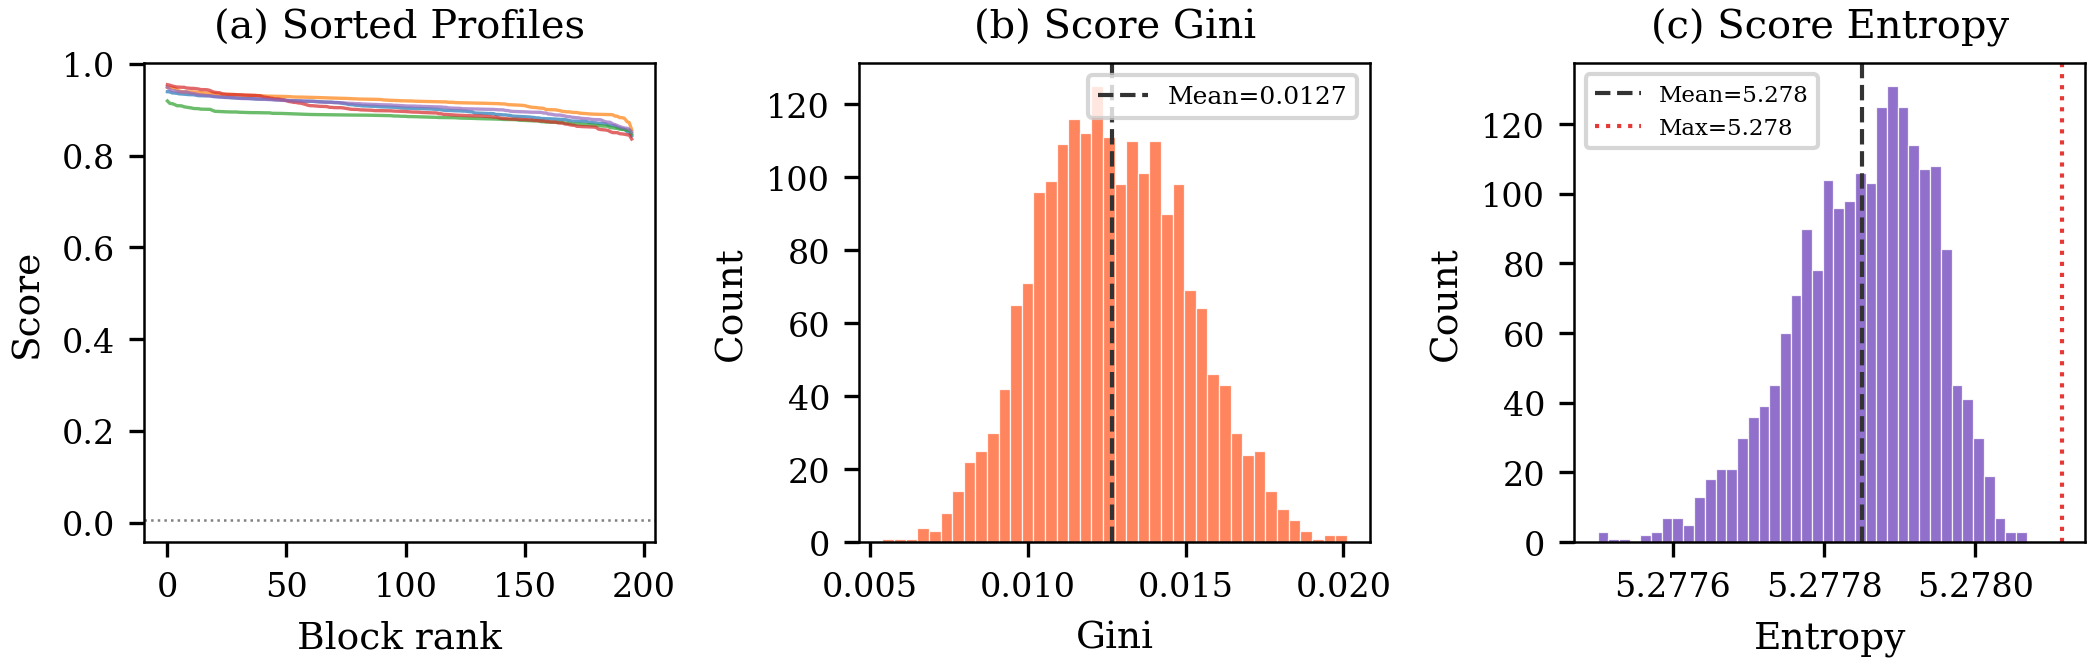
\includegraphics[width=\columnwidth]{figures/v2_score_distributions.png}
\caption{v2 score distributions: sorted profiles, Gini histogram, entropy histogram.}
\end{figure}

\begin{figure}[h]
\centering
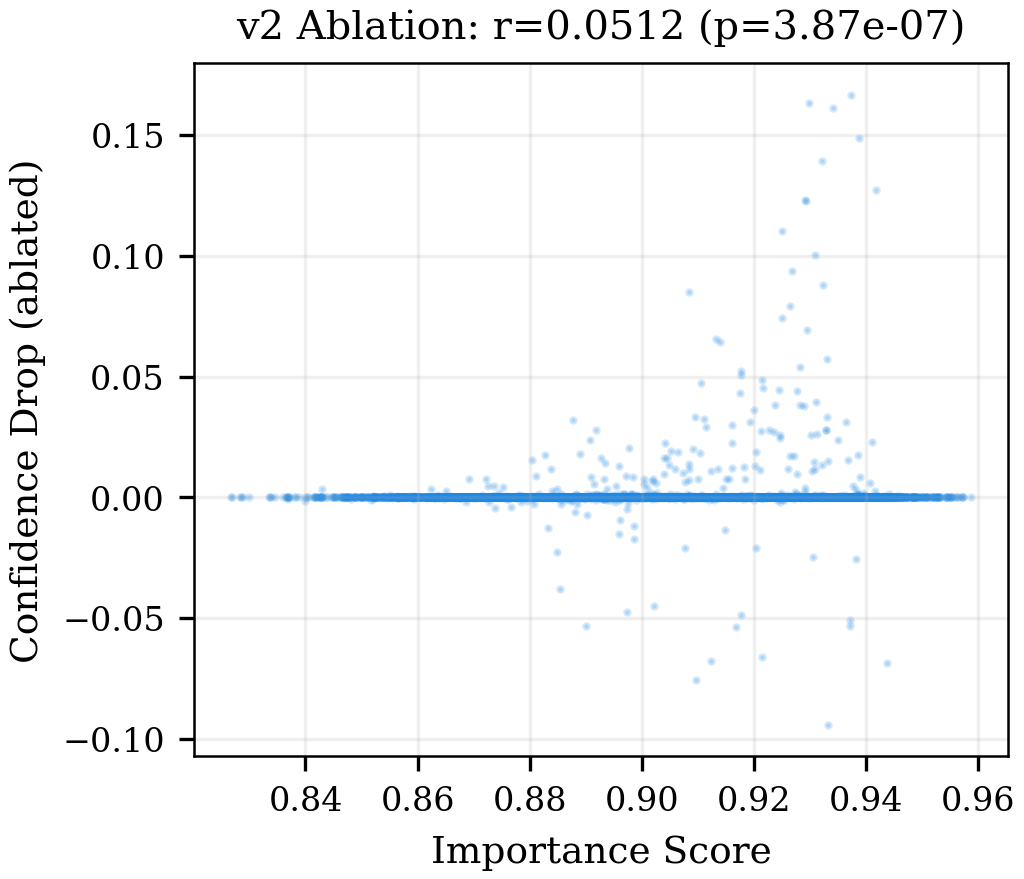
\includegraphics[width=\columnwidth]{figures/v2_ablation_corr.png}
\caption{v2 ablation correlation: $r{=}0.051$ (Pearson), $\rho{=}0.148$ (Spearman), both significant.}
\end{figure}


\end{document}
